% Minimal sebenta template generated automatically
\documentclass[11pt,a4paper]{article}
\usepackage[utf8]{inputenc}
\usepackage[T1]{fontenc}
\usepackage{lmodern}
\usepackage{geometry}
\usepackage{fancyhdr}
\usepackage{hyperref}
\usepackage{graphicx}
\usepackage{float}
\usepackage{placeins}
\usepackage{bookmark}
\usepackage{booktabs}
\usepackage{amsmath,amssymb}
\usepackage{csquotes}
\usepackage{enumitem}
\usepackage{tikz}
\IfFileExists{pgfplots.sty}{\usepackage{pgfplots}\pgfplotsset{compat=1.17}}{}

\geometry{margin=2.5cm}

% Try to include project-specific style macros (containing \exercicio, \subexercicio, etc.)
% Try multiple relative locations to be robust across different generated output paths
\IfFileExists{../../../../Teste_modelo/config/style.tex}{% Sistema de exercícios com contadores automáticos
\newcounter{exerciciocount}          % Contador principal dos exercícios
\newcounter{subexerciciocount}       % Contador dos subexercícios
\newcounter{optioncount}             % Contador das opções

% Control whether the macro prints the automatic "Exercício N." heading.
% Default: show the heading. Call \showexerciciotitlefalse to suppress.
\newif\ifshowexerciciotitle
\showexerciciotitletrue

% Macro para exercício principal
\newcommand{\exercicio}[1]{%
        \par\vspace{1.5em}% Espaçamento antes
        \refstepcounter{exerciciocount}% Incrementa contador principal
        \setcounter{subexerciciocount}{0}% Reseta contador de subexercícios
        \setcounter{optioncount}{0}% Reseta contador de opções
        % Only print the automatic heading if the flag is true
        \ifshowexerciciotitle
            \noindent\textbf{Exercício~\theexerciciocount.}\space #1\par\vspace{0.5em}%
        \else
            % When suppressed, just print the content without the heading
            #1\par\vspace{0.5em}%
        \fi
}

% Macro para subexercício
\newcommand{\subexercicio}[1]{%
    \par\vspace{0.8em}% Espaçamento menor para subexercícios
    \refstepcounter{subexerciciocount}% Incrementa contador de subexercícios
    \noindent\textbf{\theexerciciocount.\thesubexerciciocount.} #1\par\vspace{0.3em}%
}

% Macro para opção
\newcommand{\option}[1]{%
    \par
    \refstepcounter{optioncount}%
    \noindent(\alph{optioncount}) #1%
}

% Título e informações do exame
\title{1ª Questão de aula do Módulo A10: Otimização}
\author{EPRALIMA - Escola Profissional Alto Lima}

\date{}

% Cabeçalho completo do teste dentro de uma caixa simples
\newcommand{\espacoAluno}{%
    \vspace{0.5cm}
    \fbox{%
        \parbox{\textwidth}{%
            \noindent\textbf{Nome do Aluno:} \underline{\hspace{7cm}} \textbf{Turma:} \underline{\hspace{1cm}}\\[0.5cm]
            \noindent\textbf{Assinatura do Professor:} \underline{\hspace{3cm}} \hfill \textbf{Nota:} \underline{\hspace{2cm}}\\[0.5cm]
            \noindent\textbf{Assinatura do Encarregado de Educação:} \underline{\hspace{3cm}}
        }%
    }
    \vspace{1cm}
}}{%
  \IfFileExists{../../../Teste_modelo/config/style.tex}{% Sistema de exercícios com contadores automáticos
\newcounter{exerciciocount}          % Contador principal dos exercícios
\newcounter{subexerciciocount}       % Contador dos subexercícios
\newcounter{optioncount}             % Contador das opções

% Control whether the macro prints the automatic "Exercício N." heading.
% Default: show the heading. Call \showexerciciotitlefalse to suppress.
\newif\ifshowexerciciotitle
\showexerciciotitletrue

% Macro para exercício principal
\newcommand{\exercicio}[1]{%
        \par\vspace{1.5em}% Espaçamento antes
        \refstepcounter{exerciciocount}% Incrementa contador principal
        \setcounter{subexerciciocount}{0}% Reseta contador de subexercícios
        \setcounter{optioncount}{0}% Reseta contador de opções
        % Only print the automatic heading if the flag is true
        \ifshowexerciciotitle
            \noindent\textbf{Exercício~\theexerciciocount.}\space #1\par\vspace{0.5em}%
        \else
            % When suppressed, just print the content without the heading
            #1\par\vspace{0.5em}%
        \fi
}

% Macro para subexercício
\newcommand{\subexercicio}[1]{%
    \par\vspace{0.8em}% Espaçamento menor para subexercícios
    \refstepcounter{subexerciciocount}% Incrementa contador de subexercícios
    \noindent\textbf{\theexerciciocount.\thesubexerciciocount.} #1\par\vspace{0.3em}%
}

% Macro para opção
\newcommand{\option}[1]{%
    \par
    \refstepcounter{optioncount}%
    \noindent(\alph{optioncount}) #1%
}

% Título e informações do exame
\title{1ª Questão de aula do Módulo A10: Otimização}
\author{EPRALIMA - Escola Profissional Alto Lima}

\date{}

% Cabeçalho completo do teste dentro de uma caixa simples
\newcommand{\espacoAluno}{%
    \vspace{0.5cm}
    \fbox{%
        \parbox{\textwidth}{%
            \noindent\textbf{Nome do Aluno:} \underline{\hspace{7cm}} \textbf{Turma:} \underline{\hspace{1cm}}\\[0.5cm]
            \noindent\textbf{Assinatura do Professor:} \underline{\hspace{3cm}} \hfill \textbf{Nota:} \underline{\hspace{2cm}}\\[0.5cm]
            \noindent\textbf{Assinatura do Encarregado de Educação:} \underline{\hspace{3cm}}
        }%
    }
    \vspace{1cm}
}}{%
    \IfFileExists{../../Teste_modelo/config/style.tex}{% Sistema de exercícios com contadores automáticos
\newcounter{exerciciocount}          % Contador principal dos exercícios
\newcounter{subexerciciocount}       % Contador dos subexercícios
\newcounter{optioncount}             % Contador das opções

% Control whether the macro prints the automatic "Exercício N." heading.
% Default: show the heading. Call \showexerciciotitlefalse to suppress.
\newif\ifshowexerciciotitle
\showexerciciotitletrue

% Macro para exercício principal
\newcommand{\exercicio}[1]{%
        \par\vspace{1.5em}% Espaçamento antes
        \refstepcounter{exerciciocount}% Incrementa contador principal
        \setcounter{subexerciciocount}{0}% Reseta contador de subexercícios
        \setcounter{optioncount}{0}% Reseta contador de opções
        % Only print the automatic heading if the flag is true
        \ifshowexerciciotitle
            \noindent\textbf{Exercício~\theexerciciocount.}\space #1\par\vspace{0.5em}%
        \else
            % When suppressed, just print the content without the heading
            #1\par\vspace{0.5em}%
        \fi
}

% Macro para subexercício
\newcommand{\subexercicio}[1]{%
    \par\vspace{0.8em}% Espaçamento menor para subexercícios
    \refstepcounter{subexerciciocount}% Incrementa contador de subexercícios
    \noindent\textbf{\theexerciciocount.\thesubexerciciocount.} #1\par\vspace{0.3em}%
}

% Macro para opção
\newcommand{\option}[1]{%
    \par
    \refstepcounter{optioncount}%
    \noindent(\alph{optioncount}) #1%
}

% Título e informações do exame
\title{1ª Questão de aula do Módulo A10: Otimização}
\author{EPRALIMA - Escola Profissional Alto Lima}

\date{}

% Cabeçalho completo do teste dentro de uma caixa simples
\newcommand{\espacoAluno}{%
    \vspace{0.5cm}
    \fbox{%
        \parbox{\textwidth}{%
            \noindent\textbf{Nome do Aluno:} \underline{\hspace{7cm}} \textbf{Turma:} \underline{\hspace{1cm}}\\[0.5cm]
            \noindent\textbf{Assinatura do Professor:} \underline{\hspace{3cm}} \hfill \textbf{Nota:} \underline{\hspace{2cm}}\\[0.5cm]
            \noindent\textbf{Assinatura do Encarregado de Educação:} \underline{\hspace{3cm}}
        }%
    }
    \vspace{1cm}
}}{%
      % style.tex not found - proceed without project macros
    }%
  }%
}

% Provide a robust fallback for macros that might be missing in style.tex
% This attempts to include the project style first (multiple relative paths),
% and only if none exist defines minimal counters and macros safely.
\IfFileExists{../../../../Teste_modelo/config/style.tex}{% Sistema de exercícios com contadores automáticos
\newcounter{exerciciocount}          % Contador principal dos exercícios
\newcounter{subexerciciocount}       % Contador dos subexercícios
\newcounter{optioncount}             % Contador das opções

% Control whether the macro prints the automatic "Exercício N." heading.
% Default: show the heading. Call \showexerciciotitlefalse to suppress.
\newif\ifshowexerciciotitle
\showexerciciotitletrue

% Macro para exercício principal
\newcommand{\exercicio}[1]{%
        \par\vspace{1.5em}% Espaçamento antes
        \refstepcounter{exerciciocount}% Incrementa contador principal
        \setcounter{subexerciciocount}{0}% Reseta contador de subexercícios
        \setcounter{optioncount}{0}% Reseta contador de opções
        % Only print the automatic heading if the flag is true
        \ifshowexerciciotitle
            \noindent\textbf{Exercício~\theexerciciocount.}\space #1\par\vspace{0.5em}%
        \else
            % When suppressed, just print the content without the heading
            #1\par\vspace{0.5em}%
        \fi
}

% Macro para subexercício
\newcommand{\subexercicio}[1]{%
    \par\vspace{0.8em}% Espaçamento menor para subexercícios
    \refstepcounter{subexerciciocount}% Incrementa contador de subexercícios
    \noindent\textbf{\theexerciciocount.\thesubexerciciocount.} #1\par\vspace{0.3em}%
}

% Macro para opção
\newcommand{\option}[1]{%
    \par
    \refstepcounter{optioncount}%
    \noindent(\alph{optioncount}) #1%
}

% Título e informações do exame
\title{1ª Questão de aula do Módulo A10: Otimização}
\author{EPRALIMA - Escola Profissional Alto Lima}

\date{}

% Cabeçalho completo do teste dentro de uma caixa simples
\newcommand{\espacoAluno}{%
    \vspace{0.5cm}
    \fbox{%
        \parbox{\textwidth}{%
            \noindent\textbf{Nome do Aluno:} \underline{\hspace{7cm}} \textbf{Turma:} \underline{\hspace{1cm}}\\[0.5cm]
            \noindent\textbf{Assinatura do Professor:} \underline{\hspace{3cm}} \hfill \textbf{Nota:} \underline{\hspace{2cm}}\\[0.5cm]
            \noindent\textbf{Assinatura do Encarregado de Educação:} \underline{\hspace{3cm}}
        }%
    }
    \vspace{1cm}
}}{%
  \IfFileExists{../../../Teste_modelo/config/style.tex}{% Sistema de exercícios com contadores automáticos
\newcounter{exerciciocount}          % Contador principal dos exercícios
\newcounter{subexerciciocount}       % Contador dos subexercícios
\newcounter{optioncount}             % Contador das opções

% Control whether the macro prints the automatic "Exercício N." heading.
% Default: show the heading. Call \showexerciciotitlefalse to suppress.
\newif\ifshowexerciciotitle
\showexerciciotitletrue

% Macro para exercício principal
\newcommand{\exercicio}[1]{%
        \par\vspace{1.5em}% Espaçamento antes
        \refstepcounter{exerciciocount}% Incrementa contador principal
        \setcounter{subexerciciocount}{0}% Reseta contador de subexercícios
        \setcounter{optioncount}{0}% Reseta contador de opções
        % Only print the automatic heading if the flag is true
        \ifshowexerciciotitle
            \noindent\textbf{Exercício~\theexerciciocount.}\space #1\par\vspace{0.5em}%
        \else
            % When suppressed, just print the content without the heading
            #1\par\vspace{0.5em}%
        \fi
}

% Macro para subexercício
\newcommand{\subexercicio}[1]{%
    \par\vspace{0.8em}% Espaçamento menor para subexercícios
    \refstepcounter{subexerciciocount}% Incrementa contador de subexercícios
    \noindent\textbf{\theexerciciocount.\thesubexerciciocount.} #1\par\vspace{0.3em}%
}

% Macro para opção
\newcommand{\option}[1]{%
    \par
    \refstepcounter{optioncount}%
    \noindent(\alph{optioncount}) #1%
}

% Título e informações do exame
\title{1ª Questão de aula do Módulo A10: Otimização}
\author{EPRALIMA - Escola Profissional Alto Lima}

\date{}

% Cabeçalho completo do teste dentro de uma caixa simples
\newcommand{\espacoAluno}{%
    \vspace{0.5cm}
    \fbox{%
        \parbox{\textwidth}{%
            \noindent\textbf{Nome do Aluno:} \underline{\hspace{7cm}} \textbf{Turma:} \underline{\hspace{1cm}}\\[0.5cm]
            \noindent\textbf{Assinatura do Professor:} \underline{\hspace{3cm}} \hfill \textbf{Nota:} \underline{\hspace{2cm}}\\[0.5cm]
            \noindent\textbf{Assinatura do Encarregado de Educação:} \underline{\hspace{3cm}}
        }%
    }
    \vspace{1cm}
}}{%
    \IfFileExists{../../Teste_modelo/config/style.tex}{% Sistema de exercícios com contadores automáticos
\newcounter{exerciciocount}          % Contador principal dos exercícios
\newcounter{subexerciciocount}       % Contador dos subexercícios
\newcounter{optioncount}             % Contador das opções

% Control whether the macro prints the automatic "Exercício N." heading.
% Default: show the heading. Call \showexerciciotitlefalse to suppress.
\newif\ifshowexerciciotitle
\showexerciciotitletrue

% Macro para exercício principal
\newcommand{\exercicio}[1]{%
        \par\vspace{1.5em}% Espaçamento antes
        \refstepcounter{exerciciocount}% Incrementa contador principal
        \setcounter{subexerciciocount}{0}% Reseta contador de subexercícios
        \setcounter{optioncount}{0}% Reseta contador de opções
        % Only print the automatic heading if the flag is true
        \ifshowexerciciotitle
            \noindent\textbf{Exercício~\theexerciciocount.}\space #1\par\vspace{0.5em}%
        \else
            % When suppressed, just print the content without the heading
            #1\par\vspace{0.5em}%
        \fi
}

% Macro para subexercício
\newcommand{\subexercicio}[1]{%
    \par\vspace{0.8em}% Espaçamento menor para subexercícios
    \refstepcounter{subexerciciocount}% Incrementa contador de subexercícios
    \noindent\textbf{\theexerciciocount.\thesubexerciciocount.} #1\par\vspace{0.3em}%
}

% Macro para opção
\newcommand{\option}[1]{%
    \par
    \refstepcounter{optioncount}%
    \noindent(\alph{optioncount}) #1%
}

% Título e informações do exame
\title{1ª Questão de aula do Módulo A10: Otimização}
\author{EPRALIMA - Escola Profissional Alto Lima}

\date{}

% Cabeçalho completo do teste dentro de uma caixa simples
\newcommand{\espacoAluno}{%
    \vspace{0.5cm}
    \fbox{%
        \parbox{\textwidth}{%
            \noindent\textbf{Nome do Aluno:} \underline{\hspace{7cm}} \textbf{Turma:} \underline{\hspace{1cm}}\\[0.5cm]
            \noindent\textbf{Assinatura do Professor:} \underline{\hspace{3cm}} \hfill \textbf{Nota:} \underline{\hspace{2cm}}\\[0.5cm]
            \noindent\textbf{Assinatura do Encarregado de Educação:} \underline{\hspace{3cm}}
        }%
    }
    \vspace{1cm}
}}{%
      % style.tex not found - define minimal counters/macros defensively
      \makeatletter
      \@ifundefined{exerciciocount}{\newcounter{exerciciocount}}{}
      \@ifundefined{subexerciciocount}{\newcounter{subexerciciocount}}{}
      \@ifundefined{optioncount}{\newcounter{optioncount}}{}

      \newcommand{\exercicio}[1]{%
        \par\vspace{1.5em}%
        \refstepcounter{exerciciocount}%
        \setcounter{subexerciciocount}{0}%
        \setcounter{optioncount}{0}%
        \noindent\textbf{Exercício~\theexerciciocount.} #1\par\vspace{0.5em}%
      }

      \newcommand{\subexercicio}[1]{%
        \par\vspace{0.8em}%
        \refstepcounter{subexerciciocount}%
        \noindent\textbf{\theexerciciocount.\thesubexerciciocount.} #1\par\vspace{0.3em}%
      }

      \newcommand{\exercicioDesenvolvimento}[1]{\par\noindent #1\par}
      \newcommand{\option}[1]{%
        \par\refstepcounter{optioncount}%
        \noindent(\alph{optioncount}) #1%
      }
      \makeatother
    }%
  }%
}

% ========== IP-BASED TEST SYSTEM MACROS (v3.5) ==========
% Support for modular exercise inclusion with numbered headings
% Provide a boolean flag to control whether the automatic heading is shown
\makeatletter
\@ifundefined{showexerciciotitletrue}{%
    \newif\ifshowexerciciotitle
    \showexerciciotitletrue
}{}
\makeatother

% Override \exercicio to respect the \ifshowexerciciotitle flag
% When false, it prints only the content without automatic heading
\renewcommand{\exercicio}[1]{%
    \ifshowexerciciotitle
        \par\vspace{1.5em}%
        \refstepcounter{exerciciocount}%
        \setcounter{subexerciciocount}{0}%
        \setcounter{optioncount}{0}%
        \noindent\textbf{Exercício~\theexerciciocount.} #1\par\vspace{0.5em}%
    \else
        #1\par
    \fi
}

\pagestyle{fancy}
\fancyhf{}
\lhead{Módulo A10 - Otimização}
\rhead{estudo monotonia}
\cfoot{\thepage}

\title{}
\author{}
\date{}

\begin{document}
\maketitle

\section*{estudo monotonia}

\subsection*{Tipos de Exercícios}
\begin{itemize}
  \item \textbf{Monotonia Pura} --- Exercícios com funções abstratas para estudar monotonia usando derivadas.
  \item \textbf{Monotonia em Contexto Real} --- Exercícios com contextos reais onde a monotonia é usada como método de análise.
  \item \textbf{Problema Real Monotonia} --- Exercícios de problema real monotonia
\end{itemize}

\vspace{1em}

% Exercício 1: MAT_A12OTIMI_ESTU_MPU_001.tex
% Exercise ID: MAT_A12OTIMI_ESTU_MPU_001
% Module: Módulo A12 - Otimização | Concept: Estudo da Monotonia
% Type: monotonia_pura | Difficulty: 2/5
% Tags: monotonia, gráfico, ramos, linear
% Author: Professor | Date: 2025-11-26

\exercicio{
Considere o gráfico seguinte, que representa uma função $f(x)$ definida por ramos no intervalo $[0,2]$:

\begin{center}
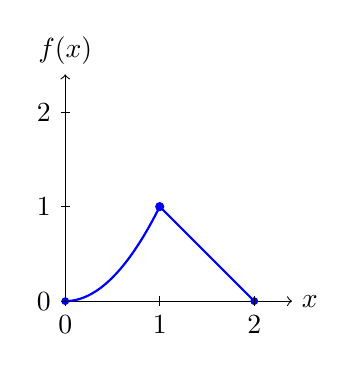
\begin{tikzpicture}[scale=1.2]
  \draw[->] (0,0) -- (2.4,0) node[right] {$x$};
  \draw[->] (0,0) -- (0,2.4) node[above] {$f(x)$};
  % ramos
  \draw[thick, blue, domain=0:1, samples=50] plot (\x, {\x*\x});
  \draw[thick, blue] (1,1) -- (2,0);
  % pontos
  \filldraw[blue] (0,0) circle (1pt);
  \filldraw[blue] (1,1) circle (1.2pt);
  \filldraw[blue] (2,0) circle (1pt);
  % marcas x
  \foreach \x in {0,1,2} \draw (\x,0.05) -- (\x,-0.05) node[below] {\x};
  % marcas y
  \foreach \y in {0,1,2} \draw (0.05,\y) -- (-0.05,\y) node[left] {\y};
\end{tikzpicture}
\end{center}
}

% f(x) = x^2 se 0 <= x < 1; f(x) = 2-x se 1 <= x <= 2
% Contexto adaptado: análise de monotonia e extremos de função por ramos quadrático/linear

\subexercicio{Indica os intervalos de $x$ onde $f(x)$ é crescente, decrescente e constante.}

\subexercicio{Qual é o valor máximo e o valor mínimo de $f(x)$ no intervalo $[0,3]$? Em que pontos ocorrem?}

\subexercicio{Interpreta o significado dos diferentes ramos do gráfico.}
\FloatBarrier

% Exercício 2: MAT_A12OTIMI_ESTU_MPU_002.tex
% Exercise ID: MAT_A12OTIMI_ESTU_MPU_002
% Module: Módulo A12 - Otimização | Concept: Estudo da Monotonia
% Type: monotonia_pura | Difficulty: 2/5
% Tags: monotonia, gráfico, ramos, linear
% Author: Professor | Date: 2025-11-26

\exercicio{
O gráfico seguinte representa uma função $g(x)$ definida por ramos no intervalo $[0,3]$:

\begin{center}
\begin{tikzpicture}[scale=1.2]
  \draw[->] (0,0) -- (3.4,0) node[right] {$x$};
  \draw[->] (0,0) -- (0,2.4) node[above] {$g(x)$};
  % ramos
  \draw[thick, red, domain=0:2, samples=50] plot (\x, {abs(\x-1)});
  \draw[thick, red] (2,1) -- (3,1);
  % pontos
  \filldraw[red] (0,1) circle (1pt);
  \filldraw[red] (1,0) circle (1.2pt);
  \filldraw[red] (2,1) circle (1.2pt);
  \filldraw[red] (3,1) circle (1pt);
  % marcas x
  \foreach \x in {0,1,2,3} \draw (\x,0.05) -- (\x,-0.05) node[below] {\x};
  % marcas y
  \foreach \y in {0,1,2} \draw (0.05,\y) -- (-0.05,\y) node[left] {\y};
\end{tikzpicture}
\end{center}
}

% g(x) = |x-1| se 0 <= x < 2; g(x) = 1 se 2 <= x <= 3
% Contexto adaptado: análise de monotonia e extremos de função por ramos valor absoluto/constante

\subexercicio{Indica os intervalos de $x$ onde $g(x)$ é crescente, decrescente e constante.}

\subexercicio{Qual é o valor máximo e o valor mínimo de $g(x)$ no intervalo $[0,5]$? Em que pontos ocorrem?}

\subexercicio{Interpreta o significado dos diferentes ramos do gráfico.}
\FloatBarrier

% Exercício 3: MAT_A12OTIMI_ESTU_MRE_001.tex
% Exercise ID: MAT_A12OTIMI_ESTU_MRE_001
% Module: Módulo A12 - Otimização | Concept: Estudo da Monotonia
% Type: monotonia_real | Difficulty: 2/5
% Tags: monotonia, gráfico, contexto_real, temperatura
% Author: Professor | Date: 2025-11-26

\exercicio{
A Maria está a fazer um bolo. A temperatura no interior do bolo foi medida ao longo do tempo, entre as 16h00 e as 16h30. O gráfico seguinte mostra como a temperatura variou durante esse período.

\begin{center}
\begin{tikzpicture}[scale=1.1]
  % Eixos
  \draw[->] (0,0) -- (7,0) node[right] {Tempo (min)};
  \draw[->] (0,0) -- (0,6) node[above] {Temperatura ($^\circ$C)};
  % Gráfico
  \draw[thick, blue, smooth] plot coordinates {
    (0,2)   % 16h00 - 20ºC
    (2,4)   % 16h10 - 60ºC
    (3,5)   % 16h15 - 100ºC (máximo)
    (5,3)   % 16h25 - 60ºC
    (6,2.5) % 16h30 - 40ºC
  };
  % Marcas no eixo x
  \foreach \x/\label in {0/0, 1/5, 2/10, 3/15, 4/20, 5/25, 6/30}
    \draw (\x,0.1) -- (\x,-0.1) node[below] {\label};
  % Marcas no eixo y
  \foreach \y/\label in {2/20, 3/40, 4/60, 5/100}
    \draw (0.1,\y) -- (-0.1,\y) node[left] {\label};
\end{tikzpicture}
\end{center}
}

\subexercicio{Durante que intervalo de tempo a temperatura do bolo esteve a aumentar?}

\subexercicio{Durante que intervalo de tempo a temperatura esteve a diminuir?}

\subexercicio{Qual foi a temperatura máxima atingida e em que minuto isso aconteceu?}

\subexercicio{Interpreta o que significa o ponto mais alto do gráfico no contexto do bolo.}
\FloatBarrier

% Exercício 4: MAT_A12OTIMI_ESTU_MRE_002.tex
% Exercise ID: MAT_A12OTIMI_ESTU_MRE_002
% Module: Módulo A12 - Otimização | Concept: Estudo da Monotonia
% Type: monotonia_real | Difficulty: 2/5
% Tags: monotonia, gráfico, contexto_real, tanque
% Author: Professor | Date: 2025-11-26

\exercicio{
Num laboratório, o nível de água num tanque foi registado ao longo de uma experiência de 30 minutos. O gráfico mostra como o nível de água variou nesse período.

\begin{center}
\begin{tikzpicture}[scale=1.1]
  % Eixos
  \draw[->] (0,0) -- (7,0) node[right] {Tempo (min)};
  \draw[->] (0,0) -- (0,6) node[above] {Nível de água (L)};
  % Gráfico
  \draw[thick, blue, smooth] plot coordinates {
    (0,1)   % 0 min - 1L
    (2,3)   % 10 min - 3L
    (4,5)   % 20 min - 5L (máximo)
    (6,2)   % 30 min - 2L
  };
  % Marcas no eixo x
  \foreach \x/\label in {0/0, 1/5, 2/10, 3/15, 4/20, 5/25, 6/30}
    \draw (\x,0.1) -- (\x,-0.1) node[below] {\label};
  % Marcas no eixo y
  \foreach \y/\label in {1/1, 2/2, 3/3, 4/4, 5/5}
    \draw (0.1,\y) -- (-0.1,\y) node[left] {\label};
\end{tikzpicture}
\end{center}
}

\subexercicio{Durante que intervalo de tempo o nível de água esteve a aumentar?}

\subexercicio{Durante que intervalo de tempo o nível de água esteve a diminuir?}

\subexercicio{Qual foi o nível máximo de água atingido e em que minuto isso aconteceu?}

\subexercicio{Interpreta o significado do ponto mais alto do gráfico no contexto da experiência.}
\FloatBarrier

% Exercício 5: MAT_A12OTIMI_ESTU_MRE_003.tex
% Exercise ID: MAT_A12OTIMI_ESTU_MRE_003
% Module: Módulo A12 - Otimização | Concept: Estudo da Monotonia
% Type: monotonia_real | Difficulty: 2/5
% Tags: monotonia, gráfico, contexto_real, temperatura, quadratica, linear
% Author: Professor | Date: 2025-11-26

\exercicio{
Durante uma experiência, a temperatura de um líquido foi registada ao longo de 2 horas. Inicialmente, o líquido aquece rapidamente, depois arrefece de forma linear. O gráfico mostra a evolução da temperatura ao longo do tempo.

\begin{center}
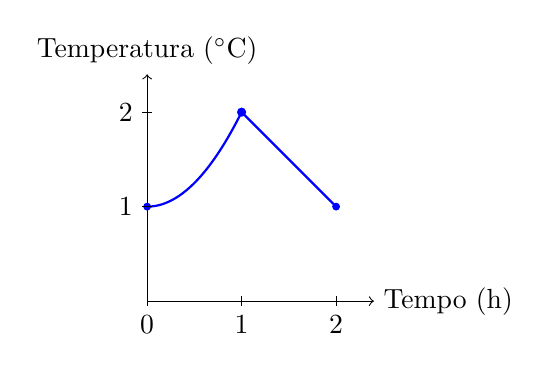
\begin{tikzpicture}[scale=1.2]
  \draw[->] (0,0) -- (2.4,0) node[right] {Tempo (h)};
  \draw[->] (0,0) -- (0,2.4) node[above] {Temperatura ($^\circ$C)};
  % ramos
  \draw[thick, blue, domain=0:1, samples=50] plot (\x, {\x*\x+1});
  \draw[thick, blue] (1,2) -- (2,1);
  % pontos
  \filldraw[blue] (0,1) circle (1pt);
  \filldraw[blue] (1,2) circle (1.2pt);
  \filldraw[blue] (2,1) circle (1pt);
  % marcas x
  \foreach \x in {0,1,2} \draw (\x,0.05) -- (\x,-0.05) node[below] {\x};
  % marcas y
  \foreach \y in {1,2} \draw (0.05,\y) -- (-0.05,\y) node[left] {\y};
\end{tikzpicture}
\end{center}
}

\subexercicio{Durante que intervalo de tempo a temperatura esteve a aumentar?}

\subexercicio{Durante que intervalo de tempo a temperatura esteve a diminuir?}

\subexercicio{Qual foi a temperatura máxima atingida e em que hora isso aconteceu?}

\subexercicio{Interpreta o significado dos diferentes ramos do gráfico no contexto da experiência.}
\FloatBarrier

% Exercício 6: MAT_A12OTIMI_ESTU_MRE_004.tex
% Exercise ID: MAT_A12OTIMI_ESTU_MRE_004
% Module: Módulo A12 - Otimização | Concept: Estudo da Monotonia
% Type: monotonia_real | Difficulty: 2/5
% Tags: monotonia, gráfico, contexto_real, velocidade, valor_absoluto, constante
% Author: Professor | Date: 2025-11-26

\exercicio{
Um ciclista inicia um percurso às 9h00. Nos primeiros 2 km, a sua velocidade varia de acordo com $v(x) = |x-1|$ (em km/h), onde $x$ é a distância percorrida em km. Depois, mantém uma velocidade constante de 1 km/h até aos 3 km. O gráfico mostra a evolução da velocidade ao longo do percurso.

\begin{center}
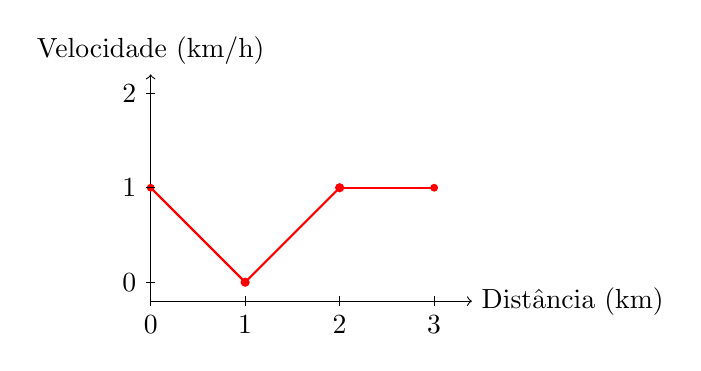
\begin{tikzpicture}[scale=1.2]
  \draw[->] (0,0) -- (3.4,0) node[right] {Distância (km)};
  \draw[->] (0,0) -- (0,2.4) node[above] {Velocidade (km/h)};
  % ramos
  \draw[thick, red, domain=0:2, samples=50] plot (\x, {abs(\x-1)+0.2});
  \draw[thick, red] (2,1.2) -- (3,1.2);
  % pontos
  \filldraw[red] (0,1.2) circle (1pt);
  \filldraw[red] (1,0.2) circle (1.2pt);
  \filldraw[red] (2,1.2) circle (1.2pt);
  \filldraw[red] (3,1.2) circle (1pt);
  % marcas x
  \foreach \x in {0,1,2,3} \draw (\x,0.05) -- (\x,-0.05) node[below] {\x};
  % marcas y
  \foreach \y in {0,1,2} \draw (0.05,\y+0.2) -- (-0.05,\y+0.2) node[left] {\y};
\end{tikzpicture}
\end{center}
}

\subexercicio{Durante que intervalo de distância a velocidade esteve a aumentar?}

\subexercicio{Durante que intervalo de distância a velocidade esteve a diminuir?}

\subexercicio{Qual foi a velocidade mínima atingida e em que ponto do percurso isso aconteceu?}

\subexercicio{Interpreta o significado dos diferentes ramos do gráfico no contexto do percurso do ciclista.}
\FloatBarrier

% Exercício 7: MAT_A12OTIMI_EXX_MRX_001.tex
% Exercise ID: MAT_A12OTIMI_EXX_MRX_001
% Module: Módulo A10 - Otimização | Concept: Estudo da Monotonia com Derivadas | Type: Monotonia em Contexto Real
% Difficulty: 4/5 (Difícil) | Format: desenvolvimento
% Tags: derivadas, modelacao, crescente, sinal_derivada, decrescente, contexto_real, monotonia, teste, automacao
% Author: Teste Automático | Date: 2025-11-26
% Status: active

\exercicio{Exercício de teste para monotonia_real}

% Solution:
% \begin{solucao}
% Solução de exemplo
% \end{solucao}
\FloatBarrier

% Exercício 8: MAT_A12OTIMI_ESTU_PRM_001.tex
% Exercise ID: MAT_A12OTIMI_ESTU_PRM_001
% Module: A12_otimizacao | Concept: estudo_monotonia
% Type: problema_real_monotonia | Difficulty: 2/5
% Tags: problema_real, otimização, monotonia
% Author: Professor | Date: 2025-11-21

\exercicio{
Numa pastelaria, a quantidade de massa (em kg) numa tigela durante a manhã foi registada. Entre as 8h e as 9h a massa cresceu de 0,5 kg para 2,5 kg (foram adicionados ingredientes). Entre as 9h e as 11h manteve-se aproximadamente constante perto de 2,5 kg (tempo de descanso/fermentação). A partir das 11h a massa diminuiu de 2,5 kg para 1,0 kg até às 12h (retirada para moldar os pães). Qual dos gráficos A, B, C ou D melhor se aproxima desta evolução ao longo do tempo?

\begin{center}
\begin{tabular}{cc}
% Gráfico A (correto: sobe 8–9, mantém 9–11, desce 11–12)
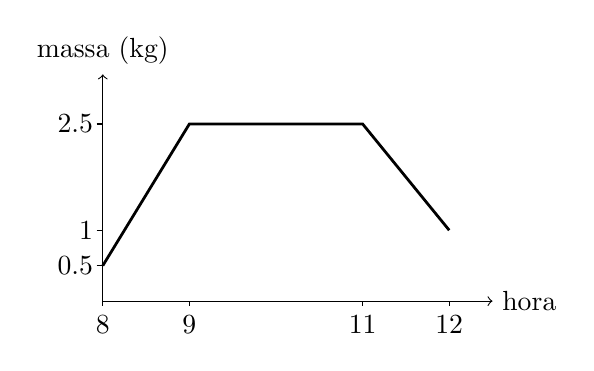
\begin{tikzpicture}[x=1.1cm,y=0.9cm]
    \draw[->] (0,0) -- (4.5,0) node[right] {hora};
    \draw[->] (0,0) -- (0,3.2) node[above] {massa (kg)};
    \draw[line width=1pt] (0,0.5) -- (1,2.5) -- (3,2.5) -- (4,1.0);
    \foreach \x/\lab in {0/8,1/9,3/11,4/12} \draw (\x,0) -- (\x,-0.07) node[below] {\lab};
    \foreach \y in {0.5,1,2.5} \draw (-0.07,\y) -- (0,\y) node[left] {\y};
    
ode at (2,-0.5) {(A)};
\end{tikzpicture}
&
% Gráfico B (cresce continuamente)
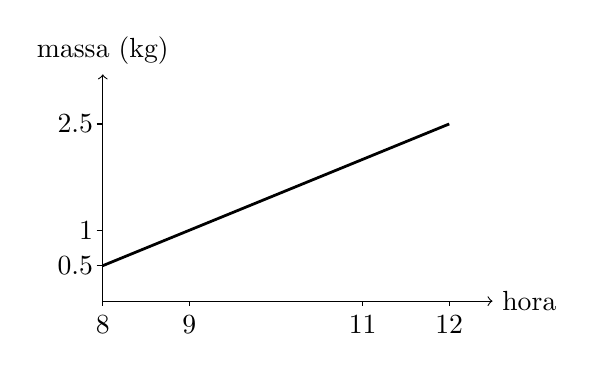
\begin{tikzpicture}[x=1.1cm,y=0.9cm]
    \draw[->] (0,0) -- (4.5,0) node[right] {hora};
    \draw[->] (0,0) -- (0,3.2) node[above] {massa (kg)};
    \draw[line width=1pt] (0,0.5) -- (4,2.5);
    \foreach \x/\lab in {0/8,1/9,3/11,4/12} \draw (\x,0) -- (\x,-0.07) node[below] {\lab};
    \foreach \y in {0.5,1,2.5} \draw (-0.07,\y) -- (0,\y) node[left] {\y};
    
ode at (2,-0.5) {(B)};
\end{tikzpicture}
\\[8pt]
% Gráfico C (desce depois sobe)
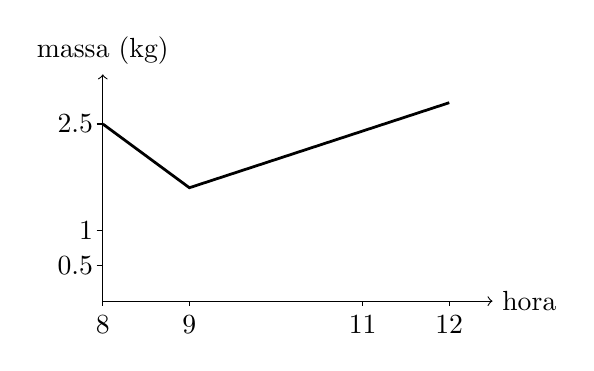
\begin{tikzpicture}[x=1.1cm,y=0.9cm]
    \draw[->] (0,0) -- (4.5,0) node[right] {hora};
    \draw[->] (0,0) -- (0,3.2) node[above] {massa (kg)};
    \draw[line width=1pt] (0,2.5) -- (1,1.6) -- (3,2.4) -- (4,2.8);
    \foreach \x/\lab in {0/8,1/9,3/11,4/12} \draw (\x,0) -- (\x,-0.07) node[below] {\lab};
    \foreach \y in {0.5,1,2.5} \draw (-0.07,\y) -- (0,\y) node[left] {\y};
    
ode at (2,-0.5) {(C)};
\end{tikzpicture}
&
% Gráfico D (praticamente constante)
\begin{tikzpicture}[x=1.1cm,y=0.9cm]
    \draw[->] (0,0) -- (4.5,0) node[right] {hora};
    \draw[->] (0,0) -- (0,3.2) node[above] {massa (kg)};
    \draw[line width=1pt] (0,2.4) -- (4,2.4);
    \foreach \x/\lab in {0/8,1/9,3/11,4/12} \draw (\x,0) -- (\x,-0.07) node[below] {\lab};
    \foreach \y in {0.5,1,2.5} \draw (-0.07,\y) -- (0,\y) node[left] {\y};
    
ode at (2,-0.5) {(D)};
\end{tikzpicture}
\end{tabular}
\end{center}
}

\subexercicio{Indique a letra do gráfico que considera correcta (A/B/C/D).}

\subexercicio{Justifique brevemente a sua escolha, referindo as partes do enunciado: "cresceu de ... a ...", "manteve-se aproximadamente constante" e "diminuiu de ... a ...".}
\FloatBarrier

% Exercício 9: MAT_A12OTIMI_ESTU_PRM_002.tex
% Exercise ID: MAT_A12OTIMI_ESTU_PRM_002
% Exercise ID: MAT_A12OTIMI_ESTU_PRM_002
% Module: A12_otimizacao | Concept: estudo_monotonia
% Type: problema_real_monotonia | Difficulty: 2/5
% Tags: problema_real, otimização, monotonia
% Author: Professor | Date: 2025-11-21

\exercicio{
Numa pastelaria, a quantidade de massa (em kg) numa tigela durante a manhã foi registada. Entre as 8h e as 9h a massa cresceu de 0,5 kg para 2,5 kg (foram adicionados ingredientes). Entre as 9h e as 11h manteve-se aproximadamente constante perto de 2,5 kg (tempo de descanso/fermentação). A partir das 11h a massa diminuiu de 2,5 kg para 1,0 kg até às 12h (retirada para moldar os pães). Qual dos gráficos A, B, C ou D melhor se aproxima desta evolução ao longo do tempo?

\begin{center}
\begin{tabular}{cc}
% Gráfico A (correto: sobe 8–9, mantém 9–11, desce 11–12)
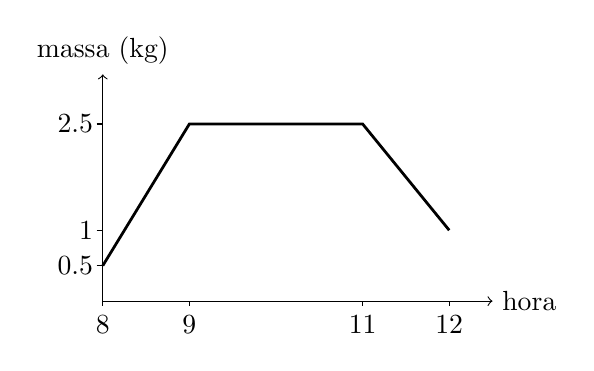
\begin{tikzpicture}[x=1.1cm,y=0.9cm]
    \draw[->] (0,0) -- (4.5,0) node[right] {hora};
    \draw[->] (0,0) -- (0,3.2) node[above] {massa (kg)};
    \draw[line width=1pt] (0,0.5) -- (1,2.5) -- (3,2.5) -- (4,1.0);
    \foreach \x/\lab in {0/8,1/9,3/11,4/12} \draw (\x,0) -- (\x,-0.07) node[below] {\lab};
    \foreach \y in {0.5,1,2.5} \draw (-0.07,\y) -- (0,\y) node[left] {\y};
    
ode at (2,-0.5) {(A)};
\end{tikzpicture}
&
% Gráfico B (cresce continuamente)
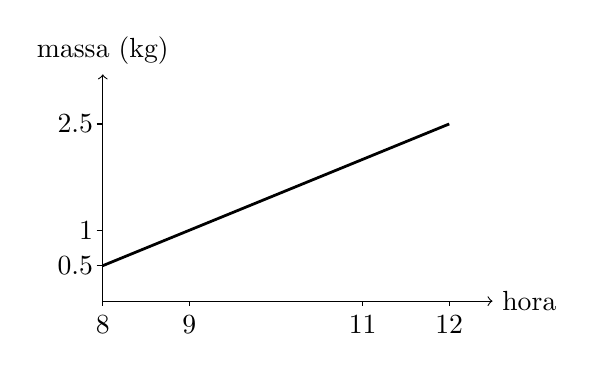
\begin{tikzpicture}[x=1.1cm,y=0.9cm]
    \draw[->] (0,0) -- (4.5,0) node[right] {hora};
    \draw[->] (0,0) -- (0,3.2) node[above] {massa (kg)};
    \draw[line width=1pt] (0,0.5) -- (4,2.5);
    \foreach \x/\lab in {0/8,1/9,3/11,4/12} \draw (\x,0) -- (\x,-0.07) node[below] {\lab};
    \foreach \y in {0.5,1,2.5} \draw (-0.07,\y) -- (0,\y) node[left] {\y};
    
ode at (2,-0.5) {(B)};
\end{tikzpicture}
\\[8pt]
% Gráfico C (desce depois sobe)
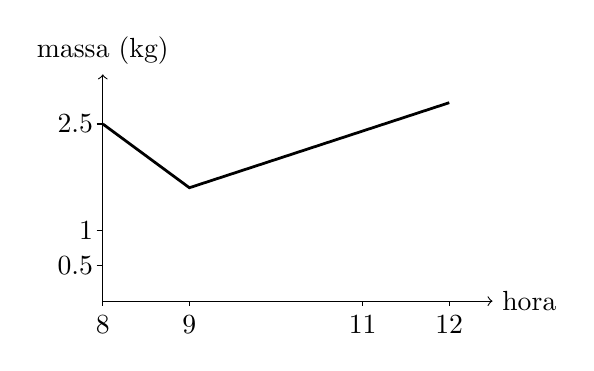
\begin{tikzpicture}[x=1.1cm,y=0.9cm]
    \draw[->] (0,0) -- (4.5,0) node[right] {hora};
    \draw[->] (0,0) -- (0,3.2) node[above] {massa (kg)};
    \draw[line width=1pt] (0,2.5) -- (1,1.6) -- (3,2.4) -- (4,2.8);
    \foreach \x/\lab in {0/8,1/9,3/11,4/12} \draw (\x,0) -- (\x,-0.07) node[below] {\lab};
    \foreach \y in {0.5,1,2.5} \draw (-0.07,\y) -- (0,\y) node[left] {\y};
    
ode at (2,-0.5) {(C)};
\end{tikzpicture}
&
% Gráfico D (praticamente constante)
\begin{tikzpicture}[x=1.1cm,y=0.9cm]
    \draw[->] (0,0) -- (4.5,0) node[right] {hora};
    \draw[->] (0,0) -- (0,3.2) node[above] {massa (kg)};
    \draw[line width=1pt] (0,2.4) -- (4,2.4);
    \foreach \x/\lab in {0/8,1/9,3/11,4/12} \draw (\x,0) -- (\x,-0.07) node[below] {\lab};
    \foreach \y in {0.5,1,2.5} \draw (-0.07,\y) -- (0,\y) node[left] {\y};
    
ode at (2,-0.5) {(D)};
\end{tikzpicture}
\end{tabular}
\end{center}
}

\subexercicio{Indique a letra do gráfico que considera correcta (A/B/C/D).}

\subexercicio{Justifique brevemente a sua escolha, referindo as partes do enunciado: "cresceu de ... a ...", "manteve-se aproximadamente constante" e "diminuiu de ... a ...".}
\FloatBarrier

% Exercício 10: MAT_A12OTIMI_ESTU_PRM_003.tex
% Exercise ID: MAT_A12OTIMI_ESTU_PRM_003
% Exercise ID: MAT_A12OTIMI_ESTU_PRM_003
% Module: A12_otimizacao | Concept: estudo_monotonia
% Type: problema_real_monotonia | Difficulty: 2/5
% Tags: problema_real, otimização, monotonia
% Author: Professor | Date: 2025-11-21

\exercicio{
Numa pastelaria, a quantidade de massa (em kg) numa tigela durante a manhã foi registada. Entre as 8h e as 9h a massa cresceu de 0,5 kg para 2,5 kg (foram adicionados ingredientes). Entre as 9h e as 11h manteve-se aproximadamente constante perto de 2,5 kg (tempo de descanso/fermentação). A partir das 11h a massa diminuiu de 2,5 kg para 1,0 kg até às 12h (retirada para moldar os pães). Qual dos gráficos A, B, C ou D melhor se aproxima desta evolução ao longo do tempo?

\begin{center}
\begin{tabular}{cc}
% Gráfico A (correto: sobe 8–9, mantém 9–11, desce 11–12)
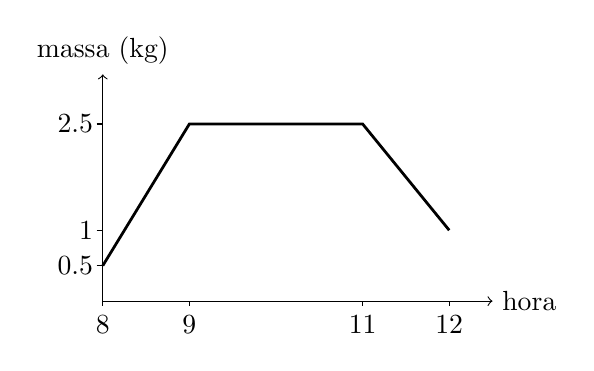
\begin{tikzpicture}[x=1.1cm,y=0.9cm]
    \draw[->] (0,0) -- (4.5,0) node[right] {hora};
    \draw[->] (0,0) -- (0,3.2) node[above] {massa (kg)};
    \draw[line width=1pt] (0,0.5) -- (1,2.5) -- (3,2.5) -- (4,1.0);
    \foreach \x/\lab in {0/8,1/9,3/11,4/12} \draw (\x,0) -- (\x,-0.07) node[below] {\lab};
    \foreach \y in {0.5,1,2.5} \draw (-0.07,\y) -- (0,\y) node[left] {\y};
    
ode at (2,-0.5) {(A)};
\end{tikzpicture}
&
% Gráfico B (cresce continuamente)
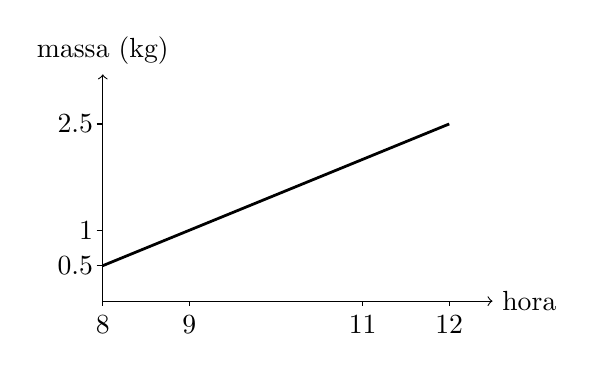
\begin{tikzpicture}[x=1.1cm,y=0.9cm]
    \draw[->] (0,0) -- (4.5,0) node[right] {hora};
    \draw[->] (0,0) -- (0,3.2) node[above] {massa (kg)};
    \draw[line width=1pt] (0,0.5) -- (4,2.5);
    \foreach \x/\lab in {0/8,1/9,3/11,4/12} \draw (\x,0) -- (\x,-0.07) node[below] {\lab};
    \foreach \y in {0.5,1,2.5} \draw (-0.07,\y) -- (0,\y) node[left] {\y};
    
ode at (2,-0.5) {(B)};
\end{tikzpicture}
\\[8pt]
% Gráfico C (desce depois sobe)
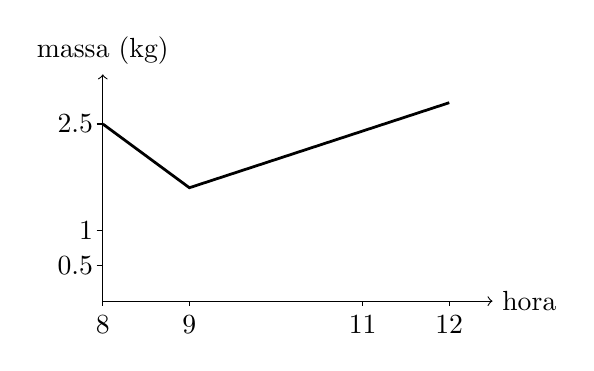
\begin{tikzpicture}[x=1.1cm,y=0.9cm]
    \draw[->] (0,0) -- (4.5,0) node[right] {hora};
    \draw[->] (0,0) -- (0,3.2) node[above] {massa (kg)};
    \draw[line width=1pt] (0,2.5) -- (1,1.6) -- (3,2.4) -- (4,2.8);
    \foreach \x/\lab in {0/8,1/9,3/11,4/12} \draw (\x,0) -- (\x,-0.07) node[below] {\lab};
    \foreach \y in {0.5,1,2.5} \draw (-0.07,\y) -- (0,\y) node[left] {\y};
    
ode at (2,-0.5) {(C)};
\end{tikzpicture}
&
% Gráfico D (praticamente constante)
\begin{tikzpicture}[x=1.1cm,y=0.9cm]
    \draw[->] (0,0) -- (4.5,0) node[right] {hora};
    \draw[->] (0,0) -- (0,3.2) node[above] {massa (kg)};
    \draw[line width=1pt] (0,2.4) -- (4,2.4);
    \foreach \x/\lab in {0/8,1/9,3/11,4/12} \draw (\x,0) -- (\x,-0.07) node[below] {\lab};
    \foreach \y in {0.5,1,2.5} \draw (-0.07,\y) -- (0,\y) node[left] {\y};
    
ode at (2,-0.5) {(D)};
\end{tikzpicture}
\end{tabular}
\end{center}
}

\subexercicio{Indique a letra do gráfico que considera correcta (A/B/C/D).}

\subexercicio{Justifique brevemente a sua escolha, referindo as partes do enunciado: "cresceu de ... a ...", "manteve-se aproximadamente constante" e "diminuiu de ... a ...".}
\FloatBarrier

% Exercício 11: MAT_A12OTIMI_EXX_PRM_001.tex
% Exercise ID: MAT_A12OTIMI_EXX_PRM_001
% Module: Módulo A10 - Otimização | Concept: Estudo da Monotonia com Derivadas | Type: Problema Real Monotonia
% Difficulty: 2/5 (Fácil) | Format: desenvolvimento
% Tags: decrescente, otimização, crescente, sinal_derivada, monotonia, problema_real, teste, automacao
% Author: Teste Automático | Date: 2025-11-26
% Status: active

\exercicio{Exercício de teste para problema_real_monotonia}
\FloatBarrier

% Exercício 12: MAT_A12OTIMI_EXX_PRM_002.tex
% Exercise ID: MAT_A12OTIMI_EXX_PRM_002
% Module: Módulo A10 - Otimização | Concept: Estudo da Monotonia com Derivadas | Type: Problema Real Monotonia
% Difficulty: 4/5 (Difícil) | Format: desenvolvimento
% Tags: decrescente, otimização, monotonia, sinal_derivada, crescente, problema_real, teste, automacao
% Author: Teste Automático | Date: 2025-11-26
% Status: active

\exercicio{Exercício de teste para problema_real_monotonia}
\FloatBarrier

\end{document}
